% using Elseveir template per https://www.elsevier.com/authors/author-schemas/latex-instructions
% model paper: Dynamic effects of teacher turnover on the quality of instruction (2016)
%   Hanushek et al
%   from Economics of Education Review
% https://www.nber.org/papers/w22472

% secondary model paper: The effects of economic policy and political uncertainties on economic activities
% Gholipour, 2019
% https://www.sciencedirect.com/science/article/pii/S0275531918306081
\documentclass[review]{elsarticle}

\usepackage{amsmath}
\usepackage{lineno,hyperref}
\usepackage{booktabs}
\usepackage{graphicx}
\usepackage{hyperref}
\usepackage{siunitx}
\usepackage{tabularx}
\usepackage{threeparttable}  
\usepackage{tikz}

% ref: https://tex.stackexchange.com/questions/19390/how-do-you-download-packages-for-texworks-on-windows-7
% ref: https://tex.stackexchange.com/questions/47418/siunitx-specifying-custom-command-as-input-symbol
\newcommand{\sym}[1]{\rlap{#1}}

\bibliographystyle{elsarticle-num}
\graphicspath{{../alt-ed-survey/figures-and-tables}}
\journal{Journal of \LaTeX\ Templates}
\modulolinenumbers[5]
\sisetup{
    detect-mode,                        %%% not grammatical
    group-digits            = false ,   %%% not grammatical
    input-signs             = ,         %%% not grammatical
    input-symbols           = ()[]-+* , % specifying \sym here does not work  %%% not grammatical
    input-open-uncertainty  = ,         %%% not grammatical
    input-close-uncertainty = ,         %%% not grammatical
    table-align-text-post   = false     %%% not grammatical
}
\usetikzlibrary{calc,matrix}

\begin{document}
\begin{frontmatter}

    \title{
        Dynamic Effects of H-1B and Section 127 Policy on Higher Education
        % \tnoteref{titlenotes}
    }
    % \tnotetext[titlenotes]{
    %     Go to \url{https://github.com/Vandivier/research-dissertation-case-for-alt-ed/tree/master/papers/}
    %     for additional materials including the online appendix,
    %     survey data, and data analysis source code.
    % }

    \author[mymainaddress]{John Vandivier} % \fnref{authorlinefootnote}}
    \address[mymainaddress]{4400 University Dr, Fairfax, VA 22030}
    \ead{jvandivi@masonlive.gmu.edu}

    \begin{abstract}
        % word count: 206
        % Hanushek model abstract word count: 151
        % ref: simple regression claim: `reg totalen employer_assistance_1'
        Section 127 of the United States Internal Revenue Code provides for a tax deduction to employers that provide employee educational assistance.
        Section 127 assistance creates an income effect, so, surprisingly,
        the historical passage is superficially associated with reduced growth in enrollment for higher education.
        Further, a simple regression of the inflation-adjusted tax-deductible limit of employer assistance on higher education enrollment indicates a significant negative correlation.
        These counterintuitive findings raise concerns that omitted variables bias estimates of the effectiveness of Section 127 assistance.
        After taking extensive steps to account for dynamic economic conditions and H-1B, veteran education, and federal loan policies,
        analysis robustly identifies positive marginal employer assistance effects on enrollment.
        The linear and total effects of interest remain negative over the main period of analysis from 1992 through 2017.
        In the preferred dynamic model, given a steady-state,
        the period-over-period effect of interest from a one thousand dollar increase to real employer assistance would be to increase total enrollment by about 7.45 million students.
        H-1B inclusion was motivated as a control, but it turns out to be a comparatively preferred policy instrument for enrollment and other policy interests.
        Results are validated using vector autoregression (VAR), dynamic ordinary least squares (DOLS), and instrumental variable (IV) analysis.
    \end{abstract}

    \begin{keyword}
        education economics, section 127, tuition assistance, veteran benefits, h-1b, debt crisis, dols, visa, immigration, autoregression %%% not grammatical
        \MSC[2010] % TODO
    \end{keyword}
\end{frontmatter}

\pagebreak
\linenumbers

\section{Introduction}
% TODO: basic time series graph.
% enrollment, loans, prices, and policy states over time are candidates.
The passage of Public Law 95-600 in 1978 created Section 127\cite{plaw95_600_1978}.
Section 127 provides for a limited employer tax deduction for the transfer of money to an employee for educational purposes.
This paper tests the hypothesis that the causal effect of Section 127 employer assistance on total university enrollment is positive.
Regression in this paper controls extensively for dynamic policy and economic variation,
then investigates robustness and Granger causality across multiple specifications.
Results show that employer assistance has a positive marginal effect on enrollment and negative linear and total effects.
H-1B visa policy is a comparatively effective policy instrument for enrollment, national student loan debt, and the price of education.
The failure of several simple theories to successfully explain the observation of enrollment slowdown in the late 1970s and 1980s further motivates the present study.

\subsection{Simple Supply-Side Explanations}
One hypothesis is that there is an adjustment period between the creation of Section 127 and widespread employer provision of the newly deductible benefit.
Allowing for a 3 or 5 year lag around the passage of Public Law 95-600 fails to harmonize observed enrollment slowdown with the expected increase to demand.
Across the eight five-year periods from 1970 to 2010, the five-year public enrollment growth rate was above 9 percent half of the time.
Two of the four low-growth intervals occurred immediately after the 1978 creation of Section 127.
The period just prior, from 1970-1975, saw the highest growth in enrollment across those eight periods.

Surveys of employers provide further data on employer provision of educational assistance over time.
Cappelli identifies three employer surveys from 1992 and 1993, which indicate that at least 86 percent of surveyed employers provided educational assistance\cite{cappelli2004employers}.
These early surveys consist of samples of convenience.
Nevertheless, further considerations lead Cappelli to conclude that a substantial majority of employers offered such plans over his period of analysis from about 1990 to 2004.
The provision of this kind of benefit remains common in later years.
In 2013, SHRM reported that 61 percent of employers offer tuition assistance\cite{cherry2014rejuvenating}.
In 2017, World at Work found that 85 percent of employers offered such a benefit,
with another 7 percent offering non-reimbursement tuition assistance, such as upfront tuition discounts\cite{talentculture_2018}.

In summary, the simplistic hypothesis of lagged or bottlenecked employer support for Section 127 fails to solve the problem,
motivating more complex analysis carried out in this paper.

\subsection{Simple Demand-Side Explanations}
A simple regression of real employer assistance on enrollment may yield a significant negative correlation wholly due to consumer effects.
The factual claim of decreasing market demand is consistent with observation, but it began before the passage of Section 127.
Falling average tuition and fees are observed for all institutions from 1972 to 1980.
The college-age enrollment percent does not increase substantially from 1970 to 1980.
Higher education prices increase after 1980, as do the college-age enrollment percentage and total enrollment.

Because the decline in demand predates the passage of Section 127, the cause of decline must be located elsewhere, at least in part.
Simplistic demand-side identification of the effects of employer assistance fails due to omitted variable bias.
Important omitted variables include controls for inflation, the price of education, and relevant policy changes.
Immigration, veteran education, and federal lending policy undergo fundamental changes in proximity to 1978 and in years later.
Sufficient identification of the effect of Section 127 must account for changes in these variables over time.

\section{Empirical Model}

This paper takes multiple steps to ensure robustness and analytical completeness.
The final results are consistent across three empirical specifications.
In addition to the variable of interest, this paper tests two other left-hand variables.
Testing these two secondary dependent variables of interest improves confidence in the theoretical and applied soundness of the conclusion.

Total postsecondary enrollment in the United States is the dependent variable.
The Section 127 policy effect is the right-hand parameter of interest in the first two specifications.
Equation \ref{eq1} is the first specification of interest. This model is an ordinary least squares model.
Here, $\alpha$ is a $1*k$ vector of coefficients,
and $V$ is a $k*1$ vector of annually observed independent variables.

% time-invarient coefficients.
% all betas are linear coefficients of their respective independent variables
% nonlinear effects are capture with exponential transforms as distinct independent variables.
% OLS
\begin{equation}
    % alternatively, longer-form:
    % Y_t = \beta_1X_{1t}+\beta_2X_2...+\beta_kX_k+e
    Y_t = \alpha{V_{t}}+u_t
    \label{eq1}
\end{equation}

Policy variables exist for federal lending policy, veteran education benefits, and H-1 Visa policy.
Two additional non-policy variables are controls for time, in years,
and the real price of university tuition plus mandatory fees.

Equation \ref{eq2} describes the next specification.
This model follows the Anderson–Hsiao pattern\cite{anderson1981estimation} with the lagged variable of interest as an instrument.
This specification investigates concerns of potential endogeneity in the dependent variable.
It is both an instrumental variable model and also a dynamic ordinary least squares (DOLS) model.

% DOLS
% ref: http://www3.grips.ac.jp/~yamanota/Lecture%20Note%208%20to%2010%202SLS%20&%20others.pdf
% could be important to acknowledge that "you must be aware that the standard errors from the two-step procedure
%   are incorrect, usually smaller than the correct ones" per supra
%   but in our case beta of interest isn't importantly different between preferred DOLS and non-IV transform
% ref: https://www-jstor-org.mutex.gmu.edu/stable/2287517?seq=2#metadata_info_tab_contents
% ref: preferred dols model from analysis-9-dols-reg-table.do
% note: Dickey-Fuller test for the presence of a unit root
%   would be an alternative, or additional, way to check for dependent var endogeneity
\begin{subequations}
    \begin{equation}
        \Delta{Y_t} = \beta{W_{t}}+B{z_t}+e_t
        \label{eq2}
    \end{equation}
    \begin{equation}
        z = \delta{W_{t}}+D{Y_{t-2}}+g_t
        % I think this is a better derivation but I'm not sure if it's completely correct:
        % z = \hat{Y}_{t-1} = \delta{W_{t}}+D{Y_{t-2}}+g_t
        \label{eq3}
    \end{equation}
\end{subequations}

Here, $\beta$ is a $1*l$ vector of coefficients,
and $W$ is an $l*1$ vector of annually observed independent variables.
$z$ is the instrument, and it is a projection of lagged enrollment derived from twice-lagged enrollment.
Equation \ref{eq3} explicitly derives $z$.
% B is the particular explanatory coefficient for $z$.
% lowkey B assumes invariance over time but let's not talk about it

$l$ is a direct transformation of $k$ from Equation \ref{eq1}.
$l$ contains five variations of each variable in $k$.
The first variation is the non-transformed value.
The other variations include the first and second lags and differences for each variable in $k$.
% In Equation \ref{eq3},
% $\delta$, $D$, and $g$ fill modelling roles analgous to $\beta$,
% $B$, and $e$ from Equation \ref{eq2}.

The third specification is a vector autoregression (VAR) model.
Six related models follow this general specification.
Equation \ref{eq:applied_naiive_var} is the first model in this family.
It is a two-variable case of that specification.
This model is similar to the previous non-VAR
specifications because it models the effect of
real employer assistance on total enrollment.
A second model follows the same form,
but the independent variable is H-1B visa issuance,
instead of Section 127 assistance.

\begin{subequations}
    \begin{equation}
        v_t = \alpha_0 + \alpha_1{v_{t-1}} + \alpha_2{v_{t-2}} + ... + \alpha_i{v_{t-i}} + u_t
        \label{eq:univariate_var}
    \end{equation}
    \begin{equation}
        V_t = \alpha_0 + \alpha_1{v_{1, t-1}} + \alpha_2{v_{2, t-1}} + ... + \alpha_{ik-1}{v_{k-1, t-i}} + \alpha_{ik}{v_{k, t-i}} + u_t
        \label{eq:naiive_multi_var}
    \end{equation}
    \begin{equation}
        Y_t = \sigma_k{V_{kt}}+e_t
        \label{eq:applied_naiive_var}
    \end{equation}
\end{subequations}
% TODO: maybe use stata built-in Granger causality Wald tests

Equation \ref{eq:univariate_var} is a univariate autoregression.
Dependent and independent variables are uniformly represented by $v_t$.
An ordinary least squares function of $i$ lags explains the current-period value of the variable in the univariate regression.
Equation \ref{eq:naiive_multi_var} extends this operation to $k$ variables.
Notice that $V_t$ is not a $k*1$ vector of univariate $v_t$.
Instead, it is a $k*k$ multivariate vector, plus a constant and an error term.

Equation \ref{eq:applied_naiive_var}
obtains $V_t$ as specified in Equation \ref{eq:univariate_var}
for all variables in $k$,
then fits an ordinary least squares model across $V_kt$ to explain the current-period dependent variable, $Y_t$.
Section 127 effects turn out to be insignificant in the specification described by Equation \ref{eq:applied_naiive_var},
but H-1B effects are significant.
As a result, all four remaining VAR equations use H-1B issuance as the independent variable.

% another good article from david, other than cited: https://blog.stata.com/2016/08/09/vector-autoregressions-in-stata/
% Lucas critique of VAR https://ocw.mit.edu/courses/economics/14-384-time-series-analysis-fall-2013/lecture-notes/MIT14_384F13_lec12and13.pdf
Two of the four remaining models are three-variable extensions of the prior specification.
These two models extend Equation \ref{eq:applied_naiive_var} by adding a second stage response.
In the first case, the second-order response is federal student loan debt.
In the second case, the second-order response is the price of higher education.
David Schenk suggests Cholesky decomposition as a method of generating an ordered impulse-response function from a VAR\cite{schenck_2016}.
Equations \ref{eq:make_structural_shocks} and \ref{eq:link_covariance_error} describe Cholesky identification.

\begin{subequations}
    \begin{equation}
        e_t = Bu_t
        \label{eq:make_structural_shocks}
    \end{equation}
    \begin{equation}
        \Sigma = E(e_t e_t')
        = E(Bu_tu_t'B')
        = B E(u_t u_t') B'
        = B B'
        \label{eq:link_covariance_error}
    \end{equation}
\end{subequations}

% I think $u_t$ is a vector and not a matrix right...?
The left-hand error term in Equation \ref{eq:make_structural_shocks}, $e_t$,
is the same as in Equation \ref{eq:applied_naiive_var}.
The right-hand of Equation \ref{eq:make_structural_shocks} defines $B$,
which is a matrix
Now $u_t$ is defined, which represent structural, or uncorrelated, error.
Endogenous error in $B$ allows us to trace out the effects of arbitrary innovation
in some variable in $V_k$.

The reduced form $BB'$ in Equation \ref{eq:link_covariance_error} matches many matrices.
A unique solution is identified by selecting the lower-triangle matrix which satisfies
the equality statement with $\Sigma$, the covariance matrix of the errors.
This arbitrary selection is isomorphic to stipulating a causal direction of effect on the variables in the VAR.
This is called a Cholesky ordering.
Stipulating a Cholesky ordering allows assessment of fit regarding the causal stipulation,
which amounts to evidence for or against causality.
It ends up being an analytical tool in this paper.
The variable orderings selected are theoretically grounded.

The last two models in the six-model VAR family are also simple two-factor VAR models.
These models test the hypothesis that enrollment effects are extraneous
to the effects of H-1B policy on student loans and the price of higher education.
The form of these models follows the specification in Equation \ref{eq:applied_naiive_var},
but the independent and response variables are different.
H-1B issuance is the independent variable.
The response variable is federal student loan debt in one case.
The price of higher education is the response variable in the other case.

\section{Data}

Information on total enrollment for all degree-granting postsecondary institutions in the United States
is provided by the National Center for Education Statistics (NCES)\cite{nces_2019}.
Enrollment figures are for the fall semester of the school year.
Information on selected years from 1947 to 2028 is provided, where values for 2018 and later are projected.
The present study does not use any of the projected values.
Other data sources and policy considerations constrain the period of interest to the 27 years from 1990 to 2016.
% total enrollment: https://nces.ed.gov/programs/digest/d18/tables/dt18_303.10.asp

Personal Consumption Expenditures (PCE) data is a measure of inflation provided by the U.S. Bureau of Economic Analysis (BEA)\cite{bea_2020}.
NCES data allows the calculation of education-specific inflation\cite{nces_2017}.
NCES data is the average tuition and required fees for full-time undergraduate students across all degree-granting postsecondary institutions.
NCES provides nominal values and values adjusted for the consumer price index (CPI) for tuition.
Cost information does not include the price of room and board.
2016 is the base year for each measure of inflation.
% https://fred.stlouisfed.org/series/PCE
% https://nces.ed.gov/programs/digest/d17/tables/dt17_330.10.asp

Nominal Section 127 limits are a matter of public law.
Section 127 took effect beginning after December 31, 1978, with a nominal assistance limit of 5,000 dollars\cite{plaw95_600_1978}.
In October 1986, Pub. L. 99–514 increased the nominal assistance limit to 5,250 dollars\cite{plaw99_514_1986}.
Combining nominal assistance over time with CPI and education-specific inflation data yields two real measures of inflation.

% begin discuss veteran benefits data
Changes to veteran education benefits are also a matter of public law.
A categorical variable is used to capture the state of veteran education benefits among five possible states over the period from 1970 to 2020.
The Servicemen's Readjustment Act of 1944 is also called the G.I. Bill.
This bill is the first interesting case of veteran benefits, but it precedes the period of interest for this study.

The original bill expired in 1956\cite{glass_2010}.
This expired state is the first state represented by the veteran education state variable.
The Veterans Educational Assistance Program (VEAP) was established in 1981\cite{veteransaffairs_2017}.
The third period of interest begins in 1984 with the enactment of the Montgomery GI Bill\cite{powers_2018}.
The fourth period of interest begins in 2009 with the Post-9/11 GI Bill.

Finally, many benefits from the Forever GI Bill became effective in 2018,
with additional provisions taking effect in 2020 and 2022\cite{veteransaffairs_2020}.
This fifth policy state is too recent to be included in the period of interest.
The recent changes in veteran education benefits are a critical caveat for any attempt at forecasting or prediction outside of the period of study.

Due to constraints on the availability of other right-hand variable data,
the main period of regression analysis ranges from 1990 to 2016.
Veteran education benefits exhibit only one change during this period,
but this factor proves to be significant in the preferred model.
% GI Bill accounting https://en.wikipedia.org/wiki/G.I._Bill#Chapter_30_(Montgomery_GI_Bill)
% Variable implemented as categorical
% [state A] original bill was 1944-1984
% [state B] VEAP established 1981 https://www.benefits.va.gov/gibill/veap.asp
% [state C] Montgomery GI went into effect 1984
% [state D] Post-9/11 GI Bill went into effect for 2009 school year https://www.thebalancecareers.com/gi-bill-for-the-21st-century-3347143
% [state E] Forever GI bill rolls out new benefits starting in 2018 https://rebootcamp.militarytimes.com/education-transition/education/2017/08/16/trump-signed-the-forever-gi-bill-here-are-11-things-you-should-know/
%
% end discuss veteran benefits data

Stafford loan data is another key component of the analysis.
Stafford loan data is relevant per se.
Moreover, Stafford loan data is a broad proxy for non-military federal student aid policy.
There are two variables for Stafford loans.
The first variable is the nominal loan limit for undergraduates.
The second variable is a dummy variable.
The dummy variable indicates whether the undergraduate loan limit is the combined limit for undergraduate and graduate loans.
A policy change in 1993 grouped these limits together.
Stafford loan data is sourced from FinAid\cite{finaid_2020}.
% TODO: should I dive into an explanation for focus on undergraduate education? not doing for now.

Visa policy is a complex issue.
The number of H-1B visas issued each year is an important variable in this study.
The Immigration Act of 1990 decomposed the existing H-1 visa into distinct H-1A and H-1B categories.
Over time, H-1B1 and H-1C classifications were established,
and many other important but less relevant classifications outside of the H-1 family exist as well.
The H-1B visa is most relevant for this study because it specifically relates to the undergraduate degree.
The Immigration Act of 1990 makes available the H-1B classification for specialized workers,
or workers in a specialty occupation.
A specialty occupation is formally defined as "an occupation that requires...attainment of a bachelor's or higher degree..."

H-1 visas are a subgroup of nonimmigrant visas.
Nonimmigrant visa award data by classification from 1987 to 2019 is provided by
the Bureau of Consular Affairs within the United States State Department\cite{bureauof_2020}.
This paper exclusively uses the most relevant H-1B visa award numbers,
but reanalysis with other visa classifications could yield statistically significant findings.
The prior H-1 visa was also a merit worker visa, but it had no formal definition of merit.
In 1989, 48,820 H-1 visas were awarded.
In 1991, 7,443 H-1A visas were awarded, and 51,882 H-1B visas were awarded.
It's plausible that the college-educated effect informally existed prior to the 1990 legislation.
One might also find small but significant effects by looking into visas outside the H-1 family.
Besides the number of actual visa awards,
an analyst could look for visa cap effects or visa policy state effects.
For example, the Pew Research Center notes that the American Competitiveness in the 21st Century Act of 2000 exempts certain entities from the H-1B cap\cite{ruiz2017key}.
% ref: https://en.wikipedia.org/wiki/H-1B_visa#H-1B_visas_issued_per_year
% more state variable food https://redbus2us.com/h1b-visa-total-cap-history-from-1990-to-current-year/
% 1952 allows unlimited merit immigration, 1990 there is a quota and degree requirement added to H-1B: https://en.wikipedia.org/wiki/H-1B_visa#Immigration_Act_of_1990
% A crackdown in 2017: https://www.investopedia.com/news/impact-trumps-h1b-visa-crackdown-5-charts/
% other policies for policy state analysis:
%   https://en.wikipedia.org/wiki/Legal_Immigration_Family_Equity_Act#V_visa
%   not sure it's relevant - https://en.wikipedia.org/wiki/Immigration_Reform_and_Control_Act_of_1986
%   https://en.wikipedia.org/wiki/H-1B_Visa_Reform_Act_of_2004
%   1986 we get h-2a and h-2b https://www.uscis.gov/ilink/docView/AFM/HTML/AFM/0-0-0-1/0-0-0-13593/0-0-0-13614.html
%   more 1986 context https://www.vox.com/2014/9/3/18080710/immigration-immigrants-reform-us
%   various visa info https://uk.usembassy.gov/visas/temporary-employment/petition-based-visas/
% 
% Open SE questions looking for more data:
% 1) https://politics.stackexchange.com/questions/52279/us-pre-1987-visa-issue-data
% 2)
% 
% Open Tweet looking for more data:
% https://twitter.com/JohnVandivier/status/1243975718649974786
% apparantly official response via twitter...cite if you dare: https://twitter.com/TravelGov/status/1243985245382283266
% they daring me: https://academia.stackexchange.com/questions/119549/can-a-tweet-be-added-to-graduate-research-proposal
% "with the caveat of ambiguous language,
%   the State Department appears to confirm tha pre-1987 data is currently digitally unavailable,
%   and perhaps permentantly unrecorded even offline."

The last data source of interest is on actual federal loans.
Actual federal loans stand in contrast to loan limits,
which are represented by the Stafford loan limit variable.
Loan limits are a policy choice, but after correcting for loan limits,
the actual amount of loans made primarily represent a demand effect.
As such, we would not want to correct for actual loans.
That would wipe out the effect of interest,
which is the demand effect attributable to various policies,
and Section 127 employer educational assistance in particular.

Instead, loan data is taken as a left-hand variable of secondary interest.
Section 127 is taken as a right-hand variable in that brief investigation.
This allows us to briefly review the relationship between Section 127 employer assistance
and the student debt crisis, a potentially related topic of importance.
The variable I use in this regard is total federal undergraduate loans,
which are extracted from a data set provided by the College Board\cite{cb_excel_2019}.
Given additional context provided by the College Board in a related report\cite{cb_trends_2019},
an analysis that decomposes federal loans by type would plausibly yield statistical refinement.
% actual undergrad loans awarded since 1990 in the excel at https://research.collegeboard.org/trends/student-aid
% My variable `Total UG Federal Loans` adapted from CB xlsx worksheet `Table 2_UG`

\section{Results}

\subsection{Multiple Regression Results}
The key independent variable is H-1B visa issuance, but at the outset,
there are two potential left-hand variables available.
Ordinary least squares (OLS) multiple regression of visa effects, time,
and tuition was run against both total enrollment and public university enrollment.
Total enrollment was more predictable than public university enrollment,
so this was selected as the preferred enrollment variable.

With total enrollment as the explained variable,
a kitchen sink multiple regression was used to select the strongest factors among other factor groups.
The total number of visas issued across classification is not significant.
Stafford loan limit variables were also identified as insignificant.
The long regression of interest has higher unadjusted explanatory power compared to kitchen sink regression.
Measures of tuition were identified as insignificant.
Table \ref{tab:table_mols} is a table of regressions which helps illustrate that, somewhat surprisingly,
real measures of employer assistance capture price and inflation effects in a preferred way
compared to using a more direct measure of tuition.

\begin{table}
    \caption{Table of Multiple Regression on Total Enrollment, Selected Variables}
    \resizebox{\columnwidth}{!}{
        
\begin{tabular}{l*{4}{c}}
    \toprule
                             &\multicolumn{1}{c}{(1)}&\multicolumn{1}{c}{(2)}&\multicolumn{1}{c}{(3)}&\multicolumn{1}{c}{(4)}\\
                             &\multicolumn{1}{c}{Enrollment}&\multicolumn{1}{c}{Enrollment}&\multicolumn{1}{c}{Enrollment}&\multicolumn{1}{c}{Enrollment}\\
    \midrule
    Montgomery GI            &  -1058516.3\sym{*}  &  -1079802.6\sym{*}  &  -1075752.6\sym{***}&   -960383.2\sym{*}  \\
                             &  (419485.4)         &  (409292.0)         &  (266842.9)         &  (353349.0)         \\
    \addlinespace
    Real Limit - Ed and PCE  &                     &      -965.9         &                     &                     \\
                             &                     &     (519.8)         &                     &                     \\
    \addlinespace
    Real Limit - Ed          &      1162.1\sym{***}&      1231.5\sym{***}&                     &      -441.6         \\
                             &     (217.1)         &     (226.0)         &                     &     (309.2)         \\
    \addlinespace
    Real Limit - Ed$^2$        &                     &                     &      0.0353\sym{***}&      0.0591\sym{***}\\
                             &                     &                     &   (0.00871)         &   (0.00730)         \\
    \addlinespace
    Real Limit - Ed$^3$        &                     &                     &-0.000000475\sym{**} &-0.000000830\sym{***}\\
                             &                     &                     &(0.000000156)         &  (9.79e-08)         \\
    \addlinespace
    Tuition CPI              &       742.2         &                     &                     &                     \\
                             &     (463.8)         &                     &                     &                     \\
    \addlinespace
    H-1 Visa                 &      -78.20\sym{**} &      -77.02\sym{**} &      -26.46         &                     \\
                             &     (22.84)         &     (22.14)         &     (19.38)         &                     \\
    \addlinespace
    H-1B Visa                &      -46.67         &      -50.77         &                     &      -17.31\sym{*}  \\
                             &     (25.16)         &     (24.96)         &                     &     (7.763)         \\
    \addlinespace
    H-1B$^2$                   &    0.000936\sym{*}  &    0.000994\sym{*}  &   0.0000856         &   0.0000427         \\
                             &  (0.000406)         &  (0.000402)         & (0.0000680)         & (0.0000339)         \\
    \addlinespace
    H-1 Non-H-1B             &       127.3\sym{**} &       123.8\sym{**} &       52.89         &                     \\
                             &     (39.18)         &     (37.78)         &     (32.95)         &                     \\
    \addlinespace
    Year                     & 416886180.7\sym{**} & 409416696.8\sym{**} & 236525780.3\sym{***}& 247765777.0\sym{***}\\
                             &(123581479.5)         &(113020808.8)         &(27200513.3)         &(32364317.1)         \\
    \addlinespace
    Year$^2$                   &   -103662.0\sym{**} &   -101789.9\sym{**} &    -58751.0\sym{***}&    -61552.8\sym{***}\\
                             &   (30771.6)         &   (28136.8)         &    (6755.8)         &    (8021.7)         \\
    \midrule
    R-sqr                    &      0.9973         &      0.9975         &      0.9970         &      0.9965         \\
    \bottomrule
    \multicolumn{5}{l}{\footnotesize Standard errors in parentheses}\\
    \multicolumn{5}{l}{\footnotesize \sym{*} \(p<0.05\), \sym{**} \(p<0.01\), \sym{***} \(p<0.001\)}\\
    \end{tabular}
    }
    \label{tab:table_mols}
\end{table}

Tuition is insignificant in model 1.
Replacing tuition with PCE and education-deflated employer assistance in model 2 identifies the latter
with significance at the 0.1 level and also improves the overall explanatory power of the model.
Real employer education assistance which is solely corrected for the price of education
is eventually preferred to the multiple-deflated measure.
This makes the education-deflated real employer assistance limit the preferred Section 127 variable.
After deciding on this variable as the preferred measure,
quadratic, cubic, and interaction transformations are investigated.
The interaction of Section 127 policy and visa effects turns out to be small in magnitude,
low in significance, and in possession of a sign which is sensitive to specification.

Model 4 is preferred out of the models presented in Table \ref{tab:table_mols}.
While model 1 has the highest r-squared value,
model 4 has an adjusted r-squared equal to model 1.
Model 4 is the result of a thorough nonlinear investigation,
while models 1 and 2 are not.
Model 3 is technically stronger but difficult to interpret.
For example, interpreting the H-1B visa policy effect is not
straightforward, both because a linear effect is missing in the model
and also because other H-1 variables are present which make pure H-1B
effect attribution impossible.

All four models are technically very strong,
but model 4 makes interpretation simple.
The linear effect of real Section 127 assistance is insignificant and negative with low confidence.
The marginal effect is highly significant and positive but decreasingly positive.
The total effect in the relevant range is also positive\footnote{
    Elimination of nonlinear effects from the preferred model acts as a robustness check,
    identifies the direction of the total effect in the relevant range,
    and maintains significance for all factors.
    The real Section 127 assistance coefficient has a point estimate of 623 in such a model,
    and the H-1B visa issuance coefficient takes a value of about -15.
}.
This indicates that a real increase to Section 127 assistance would further boost enrollment,
but such increases would be decreasingly effective.

H-1 visa effects are complex and important across specifications.
The preferred model identifies a significant negative linear effect on enrollment
from H-1B visa issuance.
There is an insignificant positive marginal effect and a total negative effect.
While the preferred model focuses on H-1B effects, analysis shows this is largely
generalizable to the H-1 family.
In fact, substituting H-1 total issuance for the linear H-1B variable improves
linear visa effect significance,
although it does not improve raw or adjusted explanatory power for the model overall.
That move also is not preferred because the linear effect and the marginal visa effects would then correspond to different measures.

Time is the most consistently significant variable across multiple regressive models.
Time, measured in years, intuitively possesses a positive linear effect and a negative marginal effect on total enrollment.
The total effect of time over the period of the analysis is also strongly positive.
A simple regression of time on total enrollment has an adjusted r-squared of about .95.
Because time is so important in explaining enrollment,
in order to facilitate robust causal analysis,
and in order to improve applied predictive modeling,
additional specifications using dynamic least squares and vector autoregression
are explored.

\subsection{Dynamic Ordinary Least Squares Results}
% ref: analysis-3-dynamic-ols.do
% TODO: another empirical model?

Dynamic ordinary least squares (DOLS) models supplement multiple regressive analysis in at least two ways.
First, autocorrelation can be removed using lagged variables in an Anderson–Hsiao adjustment\cite{anderson1981estimation}.
Second, atemporal marginal effects can be tested against marginal effects in a dynamic context,
which improves model utility in an applied context.

Table \ref{tab:table_dols} compares selected variables from two models of interest.
Selected variables include any variable which appears in both models.
The first model of interest is the preferred multiple regression with an Anderson-Hsiao adjustment.
The Anderson-Hsiao adjustment involves three changes that allow an analyst to address an issue of actual or potential autocorrelation in the dependent variable.
The first step in the adjustment is to leverage an instrumental variable regression instead of an ordinary least squares regression.
The second step is to pick a particlar instrumental variable, often called the Anderson-Hsiao estimator.
The Anderson-Hsiao estimator is a twice lagged first difference of the dependent variable.
The third step is to replace the dependent variable with the first difference of itself.
After taking these three steps, the model is removed of overlapping periods which contribute to autocorrelation over time.
The second model of interest is the preferred DOLS model.

\begin{table}
    \caption{Table of DOLS Regression on Total Enrollment, Selected Variables}
    \begin{tabularx}{\textwidth}{X}
        \centering
        
\begin{tabular}{l*{2}{c}}
    \toprule
                             &\multicolumn{1}{c}{5}&\multicolumn{1}{c}{6}\\
    \midrule
    H-1B$^2$                   &  -4.217e-06        &   7.578e-04\sym{++}\\
                             & (5.768e-05)        & (3.354e-04)        \\
    \addlinespace
    H-1B$^3$                   &                    &  -2.086e-09\sym{++}\\
                             &                    & (9.547e-10)        \\
    \addlinespace
    Real Limit - Ed          &   3.359e+02        &  -2.202e+02\sym{+} \\
                             & (5.214e+02)        & (1.014e+02)        \\
    \addlinespace
    Real Limit - Ed$^2$        &  -4.256e-04        &   5.406e-03\sym{++}\\
                             & (1.294e-02)        & (2.026e-03)        \\
    \addlinespace
    Year$^2$                   &  -2.064e+04        &  -5.706e+01\sym{*} \\
                             & (1.633e+04)        & (1.489e+01)        \\
    \midrule
    R-sqr                    &      0.5172        &      0.9252        \\
    \bottomrule
    \multicolumn{3}{l}{\footnotesize Standard errors in parentheses}\\
    \multicolumn{3}{l}{\footnotesize \sym{+} \(p<0.10\), \sym{++} \(p<0.05\), \sym{*} \(p<.01\), \sym{**} \(p<.001\)}\\
    \end{tabular}
    \end{tabularx}
    \label{tab:table_dols}
\end{table}

The preferred dynamic OLS model obtains an adjusted r-squared of about 0.85.
In contrast, the simple adjustment to the preferred multiple regression
obtains an adjusted r-squared of about 0.26.
A surprising result is that the Anderson-Hsiao estimator is insignificant
across multiple specifications, including the preferred DOLS model (p = 0.51).
A significant marginal time effect is observed in the model.
This provides evidence that the apparent dynamic autocorrelation is
mainly due to an independent time effect and other stable independent effects.

While the Anderson-Hsiao estimator is insignificant,
dropping that variable and running an ordinary regression reduces adjusted r-squared to 0.82,
but all independent factors retain significance.
This demonstrates comparative model robustness over the preferred multiple regression.
For this reason, the preferred DOLS model, with or without instrumentation,
is preferred to the preferred multiple regression identified as
model 4 in Table \ref{tab:table_mols}.

Lagged employer assistance effects are insignificant when explaining the first difference of total enrollment.
First and second differences are significant.
Current period linear and marginal effects are also significant.
The first difference and the current period marginal effect for
Section 127 assistance are both significant and positively signed.
This indicates that raising assistance,
whether in the current period or over time,
is expected to boost enrollment at the margin.
Both marginal effects follow an Inada-like pattern, where the marginal effect is decreasingly positive.
The linear effect on employer assistance is significant and negative.

I now calculate the total effect of employer assistance.
Model 6, the preferred model, is fit to the years 1992 through 2017.
The average values for the relevant independent variables over this period include
an average real assistance limit of 13942.22,
an average squared assistance limit of $2.56x10^8$,
an average first difference in assistance of -1228.18,
and an average second difference of 122.87.
Based on these values, the total effect of employer assistance over the model period is
a decrease in enrollment by about 3.34 million\footnote{
    The total effect is the rounded result of solving $X=-220.1953*13942.22+(2.56*10^8)*.0054062+1314.489*-1228.18-355.0654*122.87$.
}.
% The time-invariant effect of a hypothetical \$1,000 real increase to employer assistance would be
% a decrease to enrollment of about 0.21 million.\footnote{
% The time-invariant effect is computed as $X=-220.1953*1000+.0054062*1000*1000$.
% }.
Suppose a steady state, where Section 127 assistance has been constant for more than three periods.
In this situation, a \$1,000 increase over the next period would result in
the first and second differences both taking a value of \$1,000.
Given such a situation,
the effect of a hypothetical dynamic \$1,000 real increase to employer assistance would be
an increase to enrollment of about 7.45 million\footnote{
    The period-over-period effect from a steady state is computed as $X=-220.1953*1000+.0054062*1000*1000+1314.489*1000-355.0654*1000$.
}.
% below stata command to get mean variables for preferred dols period of analysis (n=26, 1992-2017)
% sum year employer_assistance_1 employer_assistance_2 d.employer_assistance_1 d.d.employer_assistance_1 if !missing(totalenrollment)  & !missing(d2.visa_m_h1b_1)

% I now estimate the total effect of employer assistance in three contrived examples.
% Suppose there have been three years of constant employer assistance.
% The real tax-deductable limit is valued at \$5,250.
% Suppose that in a fourth period there is a change of \$0.
% The total effect of employer assistance in this fourth period would be
% to decrease enrollment by about 1.01 million\footnote{
%     This is the rounded result of solving Y = -220.2*5250+.0054*5250*5250.
% }.
% In a second scenario, suppose that in the fourth year the real tax-deductable limit is reduced to \$0.
% The total effect of employer assistance in this fourth period would be
% to decrease enrollment by about 5.04 million\footnote{
%     This is the rounded result of solving Y = 1314.489*-5250+-355.065*-5250.
% }.
% Finally, in a third scenario, suppose real employer assistance is increased by \$2,000.
% The total effect of interest in this case would be
% to increase enrollment by about 0.61 million\footnote{
%     This is the rounded result of solving Y = -220.2*7250+.0054*7250*7250+1314.489*2000+-355.065*2000.
% }.

First-difference, lagged, and current H-1B visa effects are all signficant,
but linear visa effects are not significant.
Lagged effects are foreign to the multiple regression specification.
DOLS specification reveals significant lagged marginal effects and positive
lagged cubic effects.
A lagged linear effect is isomorphic to a first difference in this specification,
so a direct measure is omitted for collinearity,
but the first difference is positive.
The total lagged effect indicates that as lagged period visa count increases,
the expected change in current period visa issuance is both positive and eventually increasingly positive.

Other than lagged effects, dynamic visa effects are consistent with an an insightful refinement of
visa effects identified under multiple regression analysis.
For example, an insignificant positive quadratic effect is identified in the preferred ordinary multiple regression.
In the preferred DOLS, a positive marginal effect is identified with significance.
Moreover, a negative first difference is also identified with signficance.
It makes sense that forcing these related and opposing marginal effects into a single variable would lead
to insignificance in a non-dynamic specification.
Using a dynamic specification we can see that marginal effects are stable,
but they move in different directions when issuance is increased with and without respect to time.
Moreover, both of these factors face marginal effects have an attenuating higher-order counterpart.
The positive static marginal effect is attenuated by a negative cubic effect.
The negative dynamic static marginal effect is attenuated by a positive and significant second-difference coefficient.

It is important to note that DOLS models explain a slightly smaller period of analysis because of the use of lagged variables.
While the preferred multiple regression covers 27 annual samples from 1990 to 2016,
the preferred DOLS model obtains a sample size of 25 over the period from 1992 to 2016.

In summary, DOLS analysis demonstrates non-robustness in the preferred non-dynamic model,
then provides an alternative model that is significantly more robust, although it
achieves a slightly lower level of explanatory power.
DOLS analysis addresses concerns of potential autocorrelation,
finding that autocorrelation is not an important concern.
DOLS also provides rudimentary causal findings by identifying changes which are associated with results in the following period.

\subsection{Vector Autoregression Results}
% ref: analysis-4-vector-auto-reg.do
% TODO: another empirical model?

Dynamic ordinary least squares provides rudimentary causal findings,
but vector autoregression provides deeper analysis in this regard.
Vector autoregression (VAR) improves on DOLS for the specific purpose
of identifying potential natural or policy instruments.
While difference and lag effects of the first and second order were manually investigated using DOLS,
vector autoregression allows for non-manual, or unsupervised,
investigation of potentially many lags to select for the optimal period.
An analyst is then able to achieve some model confidence in both the total policy effect over time
and also the shape of how that effect will play out over time.

Multiple regression ruled out the significance of an interaction variable between
visa issuance and employer assistance,
so this analysis does not suppose that those variables are endogenous.
Instead, each is addressed as a separate potential stimulus to the response variable.
In the preferred dynamic model, visa and employer assistance effects
are the only effects that exist other than time.
As a result, each of the two VAR models are both simple, two-variable models.

For the employer assistance model,
an extended sample of 43 observations
over the period from 1974 to 2016 is used.
For the H-1B model, 24 samples over the period from 1994 to 2017 are used.
Ivanov and Kilian find that the Schwarz Information Criterion,
also called Schwarz's Bayesian information criteria (SBIC),
is the most accurate selection criterion for sample sizes less than 120\cite{ivanov2005practitioner}.
For that reason, I prefer this criterion.
Fortunately, all significant selection criteria provided by STATA unanimously agreed in the case of lag selection for both models.
Such criteria included SBIC, the likelihood ratio (LR), the final prediction error (FPE),
Akaike Information Criterion (AIC), and Hannan-Quinn Information Criterion (HQIC).
For both models, the optimal lag length is identified at two periods.
The p-value for the optimal lag was less than 0.001 for both models.

VAR results for employer assistance are directionally consistent with prior analysis.
A positive shock to employer assistance is associated with a downward parabola curve response.
The response, however, is not significant for any period, even when using a 60 percent confidence interval.

VAR results for an H-1B policy impulse are significant.
A positive shock to H-1B issuance is also associated with a downward parabola curve response.
The effect is insignificant at the 0.5 level for the first two periods,
but the reaches a significant positive effect in the third period.
The positive effect plateaus in the seventh period, then reverses,
reaching a permanent zero effect in the eleventh period.

Increased enrollment reflects an increase in demand which is associated with
increased tuition and debt both theoretically and in the present data\footnote{
    A simple regression of total enrollment on total federal loans yields a
    positive coefficient with a p-value less than 0.001 and an adjusted r-squared
    of 0.973.
    A simple regression of total enrollment on CPI-adjusted real tuition yields a
    positive coefficient with a p-value less than 0.001 and an adjusted r-squared
    of 0.915.
}.
From a policy perspective, increasing enrollment may not be desirable.
Higher education has a great return from an individual perspective, but there are several concerns from a social perspective.
Examples include concerns about grade inflation, credential inflation, experience inflation,
and the social return to education spending abound.
For example, Forbes magazine recently pointed out that the price of college is increasing almost eight times faster than wages\cite{maldonado2018price}.
Edvisors notes that the average tuition inflation rate is double the average CPI-U\cite{edvisors_2019}.
Many in the media consider the size of federal student loan debt to be a crisis.
Because H-1B policy is an enrollment instrument,
and enrollment is directly related to loans and real tuition,
further analysis investigates a downstream effect of H-1B policy on loans or real tuition.

A short regression of three variables on total enrollment
identifies a positive but insignificant (p < 0.2)
interaction between tuition and loans significantly interact.
The independent variables include total loans,
CPI-adjusted tuition,
and an interaction variable.
It is plausible that more sophisticated analysis may prove some kind of interaction exists, but even supposing significance, the correct Cholesky ordering is non-obvious.
Based on the lack of interaction, further analysis scopes loans and tuition to separate models.

\begin{figure}[h!]
    \centering
    \caption{H-1B VAR Results}
    \begin{tikzpicture}[element/.style={minimum width=1.75cm, minimum height=0.85cm}]
        \node (n1) {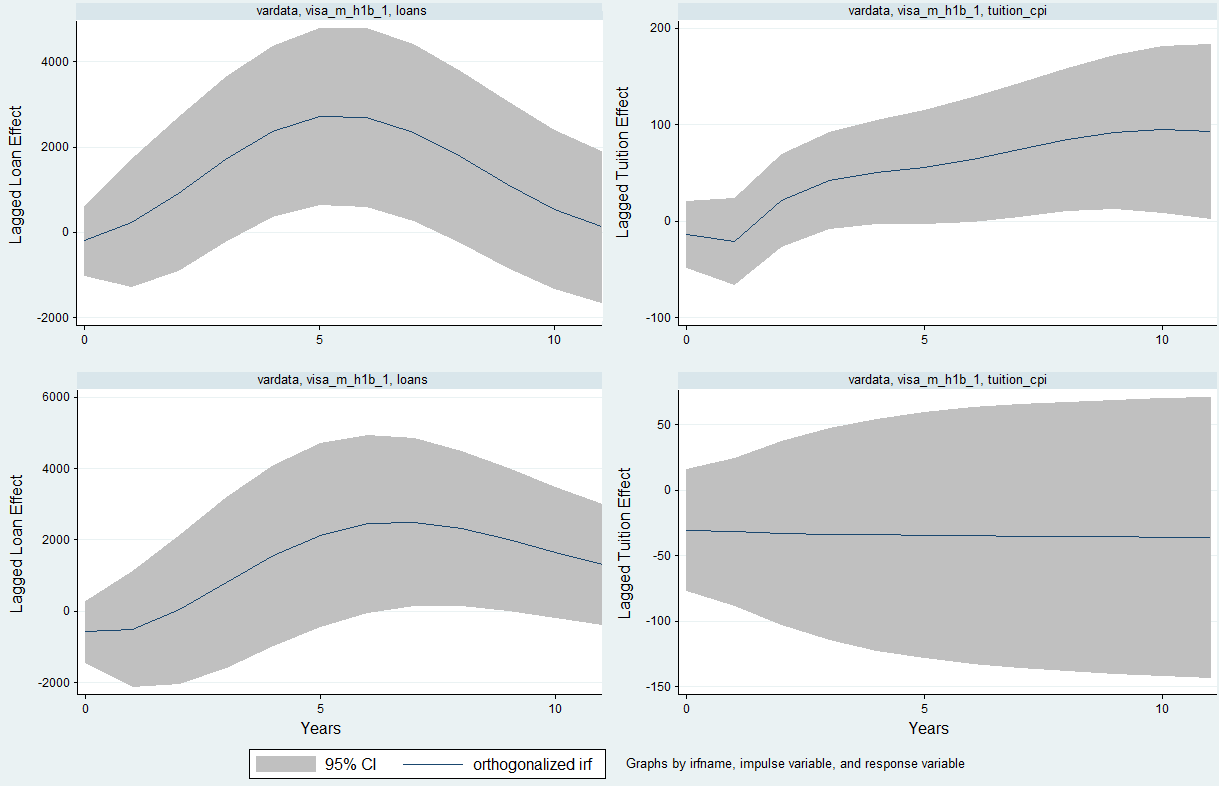
\includegraphics[width=1\textwidth]{./figures-and-tables/fig-1-var-composite.png}};
    \end{tikzpicture}
    \label{fig:var_results}
\end{figure}

Figure \ref{fig:var_results} is a graphical representation of the VAR model results.
The top row contains three-variable models of interest.
In these models, an H-1B impulse generates a first-order enrollment response.
The bottom row contains two-variable specifications that omit the intermediary enrollment response.
On the left are the loan models, and on the right are the tuition models.

The figure makes the three-variable model preference clear for tuition,
but some model statistics make the case stronger with respect to the loan models.
In the two-variable loan VAR, the r-squared for the visa variable is less than 0.89,
and the r-squared for the loan variable is less than 0.988.
In the three-variable specification, r-squared for the visa variable is greater than 0.913,
and the r-squared for the loan variable is greater than 0.989.
This confirms that the enrollment effect is model-improving rather than extraneous complexity.

Both three-variable models achieve significance at the 0.05 level.
Both three-variable models are optimized for two lags based on the SBIC selection criterion.
As previously discussed, I prefer the Schwarz Information Criterion because these models involve small sample sizes.
The loan model has a sample size of 25 over the years from 1993 to 2017.
The CPI-adjusted tuition model has a sample size of 25 over the years from 1992 to 2016.

The loan model anticipates a temporary increase in total loans,
followed by an eventual return to zero.
The tuition model allows for the same,
but it also potentially indicates the establishment of a new normal
of higher real tuition prices as a result of a one-time H-1B impulse.
We earlier noted that the interaction seems weak, but it has a positive sign.
It does not seem to be the case that a real-world shock would result in one or the other effect.
Instead, a real-world H-1B shock would be expected to cause both effects,
and these models potentially understate their effects if interaction generates higher enrollment.

In summary, vector autoregression confirms H-1B visa issuance as a Granger-causal policy instrument.
Employer assistance has the expected dynamic effect pattern, but it is insignificant in the VAR specification.
Additional analysis indicates H-1B can be leveraged not only to directly impact enrollment,
but to further impact aggregate student loans and the real price of tuition.

\section{Conclusions}

A surprising slowdown in enrollment is observed around the time Section 127 was created.
Cappelli constrains a simple slow employer adoption hypothesis by demonstrating widespread adoption as early as 1993.
Demand-side explanations do a fair job of explaining low enrollment until about 1980.
From about 1980 until about 1993, several important economic and policy variations are identified.

% Cappelli also provides evidence that employee utilization of educational benefits preferentially go to graduate students.
% This motivates hypotheses on undegraduate access.
% One reason undergraduates might lack access is because they are not being hired.
% Without a job, the undergraduate student is unable to obtain employer assistance.
% This hypothesis motivates theories about why employers began selecting for college graduates.

% The common story, with much evidence to prove it, is that the college degree is a signal of employee quality.
% but in modern times many employers are eliminating degree require

% useful lost bits.
% Employees who leverage this benefit by necessity enroll in a university.
% Willis Towers Watson estimates that fewer than 10 percent of eligible employees use tuition reimbursement benefits annually\cite{merrick_2019},
% but this remains a substantial change in demand.
%
% The original Section 127 nominal limit was \$5,000.
%
% It is surprising that 1978 is associated with a local decrease in the growth rate on both total and public university enrollment.

% \subsection{Integrating Simple Explanations}

% Cappelli provides evidence that most employers provide education benefits by 1993,
% The idea that graduate students mainly use employer education benefits motivates hypotheses around undergraduate access.
% Increasingly since the 1990s, developed economies have experienced degree inflation and experience inflation.
% Entry level positions now require a degree when previously this was not necessary, even when technology has made the work easier.
% It is possible that undergraduate access to employer benefits are reduced simply because employers increasingly hire individuals that already have the degree.
% Employers are known to value the degree as a signal of labor quality, but these days there are plenty of other, richer data sources on quality for certain professions.
% In computer programming we see some employers completely dropping the degree requirement and preferring technical interviews, digital portfolio evaluation, and other signals.
% Why, then, do other leading employers continue to require the degree?
% One answer is that the degree requirement forms an H-1B justification.
% Since the passage of the Immigration Act of 1990\cite{law1990law}, a corporation must claim a shortage of qualified specialized labor to justify an H-1B.
% The "attainment of a bachelor's or higher degree" is written into the law as a test of whether labor is qualified and specialized.
% This would motivate employers to begin requiring the degree in order to obtain cheap immigrant labor, even while knowing the degree may not be necessary.
% Such a corrected analysis is exactly what this paper completes.

% we see increasing h-1b increases loans temporarily and tuition permanently, so it's bad right? not so fast!
% h-1b labor is specialized immigrant labor, so it's beneficial for the economy. Maybe even net of above negative impacts.
% what if we could get all of the benefit of immigration without the cost of loans and tuition, credential inflation, etc?
% potential solution: change H-1B to remove the degree as meaningful. Employers are already throwing it out!
% use alternative credentials. alternative learning is adaptive and effective, cheaper and super cool. even resistant to COVID!
% the total effect of assistance in the relevant range is positive, and additional real assistance would further boost attendance.
% however, it's not obvious that increased attendance is a good thing. credential inflation, experience inflation, debt crisis.
% i fail to find evidence supporting a significant interaction between section 127 and visa policy
% however visa policy in itself is extremely important in the conversation on enrollment, credential inflation, experience inflation, and debt crisis.
% there are important caveats in this visa analysis.
% employers have recently been removing the degree requirement
% the law should also remove that requirement and boost alternative education which doesn't require a formal degree and is highly effective
% this will reduce debt, improve diversity and economic efficiency and individual skill

% maybe talk about stress and debt for why debt is important
% important to look at wages not income (which would include investments, etc, see shrm's discussion: http://www.cpepea.com/wp-content/uploads/2017/05/10-0418-Coalition-Report-on-Public-Policy-Issue-E-P-E-A_FNL.pdf)
% SHRM assessed only a single year, 2008. Shows Section 127 is mostly a Master's degree tool rn.
% 75 percentile for salaries in 2017 was 54250 https://bizfluent.com/info-10032733-percentile-salary.html
% define middle class as 50-75 percentile, lower class as under 50 percentile. break down effect by salary classification and see if it helps lower/middle
% if so, it should improve diversity of education leading to a more diverse workforce which employers crave (TM) and politicians, etc...
% Should we actually enact this policy? Effect on alternative credentials and credential inflation
% Other options like extending the benefit to repayment https://blog.shrm.org/blog/let-s-fight-the-skills-gap-by-expanding-tax-free-education-assistance
% we can also consider extending the education benefit to unaccredited education and income share agreements not just loans

% https://www.nber.org/papers/w9225.pdf 
% https://www.nber.org/digest/feb03/w9225.html

\bibliography{./BibFile}

\end{document}
